\documentclass[12pt,english]{article}
\usepackage[a4paper,bindingoffset=0.2in,%
            left=1in,right=1in,top=1in,bottom=1in,%
            footskip=.25in]{geometry}
\usepackage{blindtext}

\usepackage[english]{babel}
\usepackage[utf8]{inputenc}
\usepackage{amsmath}
\usepackage[colorinlistoftodos]{todonotes}
\usepackage{graphicx}
\usepackage{amssymb}
\usepackage[backend=bibtex]{biblatex}
\addbibresource{mybib.bib}
\usepackage[hidelinks]{hyperref}


\title{Correlation between Professional Domain and Facial Features based on Face Clustering}

\author{Bithiah Yuan}

\date{\today}

\begin{document}

\maketitle

%\begin{abstract}
%Bitcoin as an electronic payment system prevents the double-spending problem using the Proof-of-Work confirmation protocol. However, security issues arise with fast payments using Bitcoin as merchants are required to exchange their goods in a short time. We examine double-spending attacks on fast-payments and show how the attacks can be executed. Moreover, we demonstrate how the countermeasures by Bitcoin developers are either ineffective or produce additional costs for the merchants. Ultimately, we present an easy and lightweight solution for the dection of double-spending attacks in fast payments.


%\end{abstract}

\section{Introduction}
\label{sec:introduction}

\quad 
A significant source of information and attributes can be derived from the human face by non-verbal communication \cite{joo}. As a result, facial features have been studied extensively in the social-science domain to predict success in reaching reputable leadership positions. In particular, studies have shown that certain facial features contribute to higher salaries and more prestigious employments for CEOs. In application, the relationship between facial characteristics and social attributes can provide an more powerful objective indicator for organizations to idenity and select effective leaders within their domain than broad facial cues such as attractiveness and competence. Results have shown that a human judge can identify business, military, and sports leaders from their faces with above-chance accuracy. However, these results are biased and do not imply the actual leadership qualities of a person \cite{olivola}.

Caused by behaviour experiments from human judgement, the the research of the social attributes and facial features in the social-sciences are limited in scalability, consistency, and generalization. For example, prior familiarity to the faces of the study and personal preferences can affect the results. Therefore, a growing number of social trait judgment studies have been extended and refined to computer vision and machine learning research due to the capability of using massive datasets and large-scale processing capacity \cite{joo}.

Through a computational framework, \cite{joo} examined the relationship between facial traits and the social construction of leadership by a trained model that can predict the outcomes of political elections based on the perceived social attributes of a person's appearance. The results indicate that similar methods can be used to predict behavior in a broad range of human social relations, such as mate selection, job placement,and political and commercial negotiations \cite{joo}.

Clustering analysis is an unsupervised learning technique that groups data points into clusters based on their similarities. It is useful in grouping a collection of unlabeled data with similar nature into clusters. \cite{shi} investigated clustering a large number of unlabeled face images into individual identities present in the data \cite{shi}. The workflow shown in Figure\ref{fig:face}. consists of obtaining face representations of a collection of unlabeled date by a deep neural network. The choice of clustering algorithm then groups the face images according to their identity.

Motivated by the researches in computational social trait judgment and \cite{shi}, the following paper aims to examine the correlation between a person's profession based on their facial features through clustering face images. The clustering problem consists of the face representation and similarity metric of the face images and the choice of clustering algorithm \cite{shi}. Due to the importance of the underlying face representation in face clustering, this paper further compares different open-source state-of-the-art feature extraction methods based on deep learning.\\

\begin{figure}[!tbp]
 \centering
    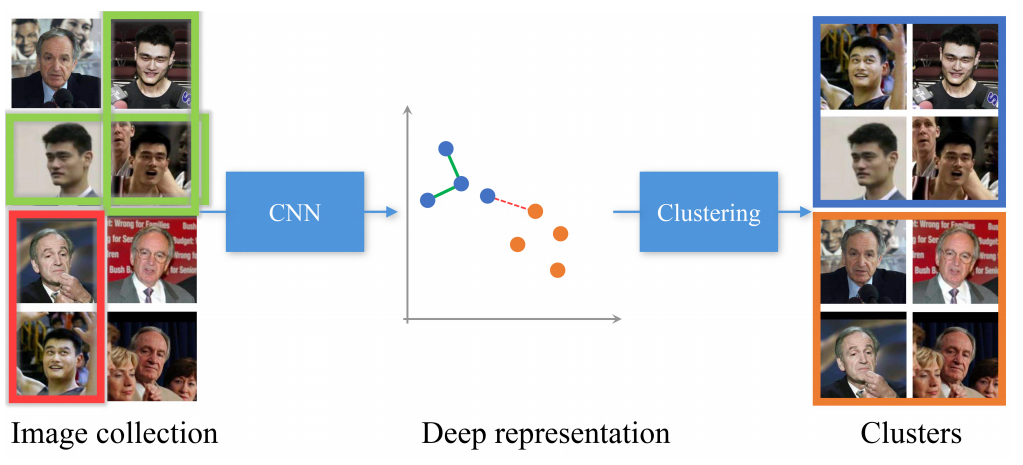
\includegraphics[width=\textwidth]{figures/otto_faceClustering_workflow.png}
    \caption{Face clustering workflow \cite{shi}}
	\label{fig:face}
\end{figure}

\section{Related Work}	

\subsection{Face Recognition}

\quad
Face recognition focuses on identifying or verifying the identity of subjects in images or videos \cite{trigueros}.\\

Face recognition systems are usually composed of the following 4 steps \cite{trigueros}: 

\begin{enumerate}
  \item \textbf{Face Detection:}\\ Detect the position of the faces in an image and returns the coordinates of a bounding box for each face as shown in Figure \ref{fig:detect}.
  \item \textbf{Face Alignment:} \\ Find a set of facial landmarks with the best affine transformation that fits a set of reference points located at fixed locations in the image as shown in Figure \ref{fig:landmark}.
  \item \textbf{Face Representation:} \\ Trasnform the pixel values of a face image into a discriminative feature vector.
  \item \textbf{Face Matching:} \\ Compute similarity scores from feature vectors.
\end{enumerate} 
 
\begin{figure}[!tbp]
  \centering
  \begin{minipage}[b]{0.49\textwidth}
    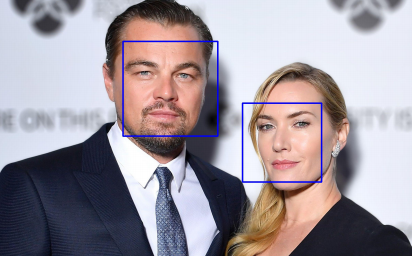
\includegraphics[width=\textwidth]{figures/face_detection.png}
    \caption{Face Detection \cite{trigueros}}
    \label{fig:detect}
  \end{minipage}
  \hfill
  \begin{minipage}[b]{0.49\textwidth}
    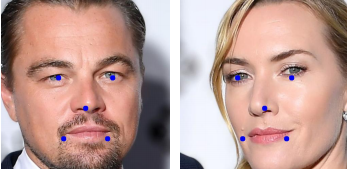
\includegraphics[width=\textwidth]{figures/landmark.png}
    \caption{Face Alignment \cite{trigueros}}
    \label{fig:landmark}
  \end{minipage}
\end{figure}

\subsection{Face Detection}

\subsubsection{Histograms of Oriented Gradients}

\quad

A traditional method for face detection is the Histograms of Oriented Gradients (HOG) descriptors, which utilizes the distribution of local intensity gradients or edge directions to characterize local object appearance and shape in an image. HOG divides the image into small grids, where each grid accumulates a histogram of gradient directions or edge orientations over the pixels of the cell. The combination of all the histogram in the cells form the face region. The cells are then normalized for better invariance to illumination, shadowing, and other variations. The normalized local histograms of image gradient orientations in a dense grid as features are then trained to classify the region of the face in an image \cite{dalal}. When encountering a HOG representation of a new face image as shown in Figure \ref{fig:obama}, the part of the image that looks most similar to a trained HOG detector as shown in Figure \ref{fig:dlibhog} will form the region of the face. 

\begin{figure}[!tbp]
  \centering
  \begin{minipage}[b]{0.35\textwidth}
    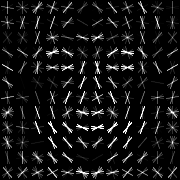
\includegraphics[width=\textwidth]{figures/hog_dlib.png}
    \caption{Trained HOG detector on multiple faces \cite{trigueros}}
    \label{fig:dlibhog}
  \end{minipage}
  \hfill
  \begin{minipage}[b]{0.45\textwidth}
    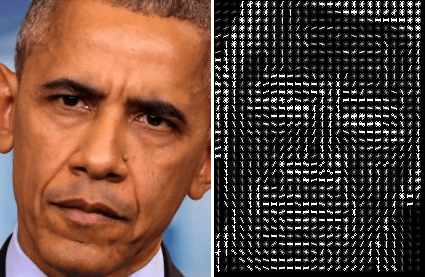
\includegraphics[width=\textwidth]{figures/face_hog.png}
    \caption{Hog representation of a face \cite{hackevolve}}
    \label{fig:obama}
  \end{minipage}
\end{figure}

\subsubsection{Multi-task Cascaded Convolutional Networks}

Another than using the tradition HOG representation and landmark detectors, face detection and alignment can also be done using CNNs. In particular, Multi-task Cascaded Convolutional Networks (MTCNN) is a widely used method to predict face and landmark location. The framework has a cascaded structure with three stages of deep CNNs shown in Figure \ref{fig:mtcnn}. \cite{zhang} 

The image is first resized to different scales to build an image pyramid and is the input of the three stages:

\begin{enumerate}
\item \textbf{Proposal Network (P-Net):} Obtains candidate windows and their bounding box regression vectors. The estimated bounding box regression vectors are used to calibrate the candidates. Then the bounding boxes are post-processed and filtered by the non-maximum suppression (NMS) algorithm to merge overlapped candidates.

\item \textbf{Refine Network (R-Net):} Rejects false candidates, calibrates the candidates with bounding box regression, and NMS candidate merge.

\item \textbf{Output Network (O-Net):} Outputs five facial landmark positions.

\end{enumerate}

Both the bounding box regression and facial landmark localization uses regression to minimize the Euclidean loss between the candidate window, landmark coordinates and the ground truth. The ground truth of the bounding boxes are the left, top, height, width of the box. The ground truth of the facial landmarks are the coordinates of the left, right eye, nose, left and right mouth corner \cite{zhang}.


\begin{figure}[!tbp]
 \centering
    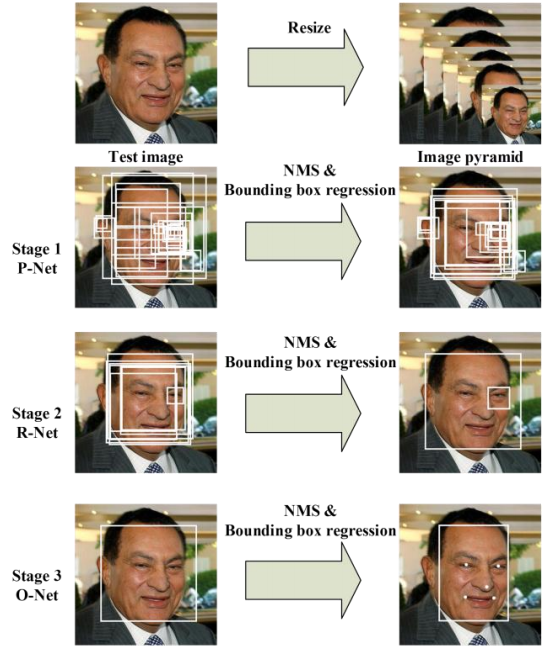
\includegraphics[width=0.7\columnwidth]{figures/mtcnn_pipeline.png}
    \caption{MTCNN: Cascaded structure with three stages of deep CNNs. \cite{zhang}}
	\label{fig:mtcnn}
\end{figure}


\subsection{Face Representation}

\subsubsection{Convolutional Neural Networks}

\quad
Face representation is conceivably the most important component in the system \cite{trigueros}. However, challenges occur in real world (in-the-wild) images due to variations ranging from head poses and illumination conditions to aging and facial expressions. Recently, deep learning methods based on convolutional neural networks (CNNs) were able to achieve very high accuracy by learning robust features due to the availability of large-scale faces in-the-wild datasets on the web \cite{trigueros}. 

Residual networks (ResNets) is a popular network architecture for face recognition. ResNets introduces a shortcut connection to learn a residual mapping which contributes to information flow across layers and allows the training of much deeper architectures \cite{trigueros}.

A common approach to training CNN models for face recognition is use a classification approach, where each face image in the training set corresponds to a class. When recognizing a new face image, the classification layer is discarded and the features of the previous layer are used as face representations. The downsides of this approach is that it doesn't generalize well to new face faces and that the representation size per face is large and inefficient \cite{schroff}.

Another approach is to learn the features for face representation directly by optimizing the distance between pairs or triplets of faces, in which the distances measure the similarity between faces \cite{trigueros} \cite{schroff}. 

\subsubsection{Triplet Loss Function}

\quad
When learning the face features directly, the choice of loss function has a great influence on the accuracy. One of the most used metric is the triplet loss function. The goal of the loss is to separate the distance between two aligned matching (positive) face images and a non-matching aligned (negative) face image by a distance margin. The result is a feature vector $f(x)$, known as embeddings, from a face image $x$ to a compact Euclidean feature space in $ \mathbb{R}^{d}$. The distance of the embeddings will be small if the faces are identical and large if the faces are distinct \cite{schroff}.


More specifically, as shown in the example in Figure \ref{fig:bale}. the distance between an anchor face image, $x_{i}^{a}$ is minimized by the loss and will be closer to all other positive face images $x_{i}^{p}$ than the negative face images $x_{i}^{n}$ where the distance is maximized by the loss. For each triplet $i$, the following condition needs to be satisfied: $$\Vert f(x_{i}^{a}) - f(x_{i}^{p}) \Vert_{2}^{2} + \alpha < \Vert f(x_{i}^{a}) - f(x_{i}^{n}) \Vert_{2}^{2} $$
where $\alpha$ is a margin that from the positive and negative pairs \cite{trigueros}.

For $N$ possible triplets, the loss being minimized is: $$ L = \sum_{i}^{N} \Big[ \Vert f(x_{i}^{a}) - f(x_{i}^{p}) \Vert_{2}^{2} - \Vert f(x_{i}^{a}) - f(x_{i}^{n}) \Vert_{2}^{2} + \alpha\Big]_{+} $$ \cite{schroff}.

\begin{figure}[!tbp]
 \centering
    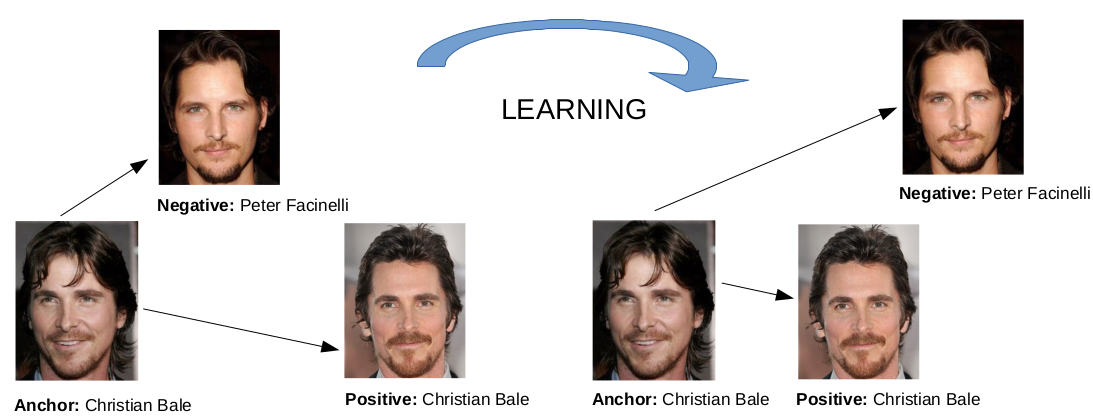
\includegraphics[width=\textwidth]{figures/triplet_loss_example.png}
    \caption{The loss of identical faces are minimized and the loss of distinct faces are maximized by the triplet loss function.}
	\label{fig:bale}
\end{figure}
 
\section{Face Representation Methods}

The following section examines open-source state-of-the-art face feature extraction methods.

\subsection{FaceNet}

\quad

FaceNet is a method that uses a deep CNN along with the GoogLeNet style Inception models and the triplet loss function to directly optimize the face embeddings. The structure of FaceNet consists of a batch input layer and a deep CNN followed by $L_{2}$ normalization, which results in the face embedding. This is followed by the triplet loss during training as shown in Figure \ref{fig:facemodel} \cite{schroff}.

%Between 100 to 200 million face images consisting of about 8 million different identities were used for training. The large dataset of labelled faces consist of various poses, illuminations, and other variations. \cite{schroff}.

\subsection{Dlib-ml}

\cite{geitgey} built a face recognition method using Dlib-ml, which is an open source library for developing machine learning software \cite{king}. \cite{geitgey} used the HOG face detector from Dlib, which the HOG representation was trained with a linear classifier (SVM) \cite{king2014}. The face representation model uses the ResNet architecture with 29 convolution layers and the triplet loss function to learn the embeddings \cite{king2017}. 

\begin{figure}[!tbp]
 \centering
    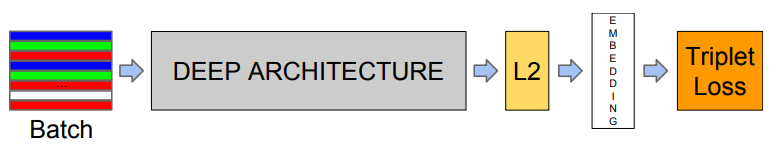
\includegraphics[width=\textwidth]{figures/facenet_model_archi.png}
    \caption{FaceNet model structure \cite{schroff}}
	\label{fig:facemodel}
\end{figure}

\section{Clustering Algorithms}

\section{Experiment}

\subsection{FaceNet}

The pre-trained model (20180402-114759) of open-source FaceNet implementation \cite{sandberg} used in the experiment was trained using the VGGFace2 dataset. The dataset contains 3.31 million images of 9131 identities, with an average of 362.6 images for each person. The images were downloaded from Google Image Search and have large variations in pose, age, illumination, ethnicity and profession. The model uses the Inception ResNet v1 architecture and has an accuracy of $99.65\%$ on the Labeled Faces in the Wild (LFW) benchmark \cite{sandberg}.

\subsection{Dlib}

A dataset of about 3 million faces and 7485 unique identities from a combination of the face scrub and VGG dataset as well as a large number of other images scraped from the internet was used for training. The pre-trained model has an accuracy of $99.38\%$ on the LFW benchmark \cite{king2017}.

\subsection{Dataset}


\subsection{Evaluation}


\section{Conclusion}

\nocite{*}

\printbibliography

\end{document}